% Chapter 3: Developer Documentation
\chapter{Developer Documentation}

\section{Introduction}

This chapter provides comprehensive technical documentation for developers who wish to understand, maintain, or extend the NutriFit system. It covers the system architecture, technologies used, database design, application components, security measures, and testing methodologies. The documentation includes detailed explanations of key implementation decisions and code examples to facilitate understanding of the system's internal workings.

\section{System Architecture}

\subsection{Overview}

NutriFit follows a modern three-tier architecture pattern consisting of the presentation layer, application layer, and data layer. Figure \ref{fig:architecture} illustrates the overall system architecture.

\begin{figure}[H]
    \centering
    \includegraphics[width=0.95\textwidth]{images/system-architecture.png}
    \caption{NutriFit System Architecture}
    \label{fig:architecture}
\end{figure}

The system architecture shown in Figure \ref{fig:architecture} demonstrates the separation of concerns across different layers. The presentation layer handles all user interactions through a responsive web interface built with React components. The application layer processes business logic through Next.js API routes, managing authentication, data validation, and plan generation algorithms. The data layer utilizes Prisma ORM for database operations, providing type-safe database access and automatic query generation. This layered architecture ensures maintainability, scalability, and clear separation between user interface, business logic, and data management.

The architecture follows the Model-View-Controller (MVC) pattern adapted for modern web applications. React components serve as the View layer, Next.js API routes function as the Controller layer, and Prisma models represent the Model layer. This separation allows independent development and testing of each layer, facilitating parallel development and easier debugging.

\section{Technologies Used}

The NutriFit system leverages modern web technologies to ensure performance, maintainability, and developer productivity. Table \ref{tab:technologies} provides a comprehensive list of technologies and their purposes.

\begin{table}[H]
\centering
\caption{Technologies and Libraries Used in NutriFit}
\label{tab:technologies}
\begin{tabular}{|p{3cm}|p{3cm}|p{7cm}|}
\hline
\textbf{Technology} & \textbf{Version} & \textbf{Purpose} \\
\hline
Next.js & 14.0.0 & React framework for server-side rendering and API routes \\
\hline
React & 18.2.0 & Frontend library for building user interfaces \\
\hline
TypeScript & 5.0.0 & Type-safe JavaScript superset for improved code quality \\
\hline
Prisma & 6.17.0 & ORM for type-safe database operations \\
\hline
SQLite & 3.x & Lightweight relational database \\
\hline
Tailwind CSS & 3.4.0 & Utility-first CSS framework for styling \\
\hline
Recharts & 2.10.0 & Charting library for data visualization \\
\hline
JWT & 9.0.2 & JSON Web Tokens for authentication \\
\hline
Bcrypt.js & 2.4.3 & Password hashing library \\
\hline
Jest & 29.7.0 & Testing framework for unit and integration tests \\
\hline
React Testing Library & 14.1.0 & Testing utilities for React components \\
\hline
\end{tabular}
\end{table}

The technology stack listed in Table \ref{tab:technologies} was carefully selected based on several criteria including performance, community support, documentation quality, and ecosystem maturity. Next.js provides server-side rendering capabilities and built-in API routes, eliminating the need for a separate backend server. TypeScript adds static typing to JavaScript, catching errors at compile-time and improving code maintainability. Prisma ORM offers type-safe database operations with automatic migration generation, significantly reducing development time and potential runtime errors.

\section{Database Design}

\subsection{Overview}

The database schema is designed to efficiently store user data, health profiles, meal and exercise logs, generated plans, and related information while maintaining data integrity and supporting complex queries. Figure \ref{fig:er-diagram} shows the Entity-Relationship diagram of the database.

\begin{figure}[H]
    \centering
    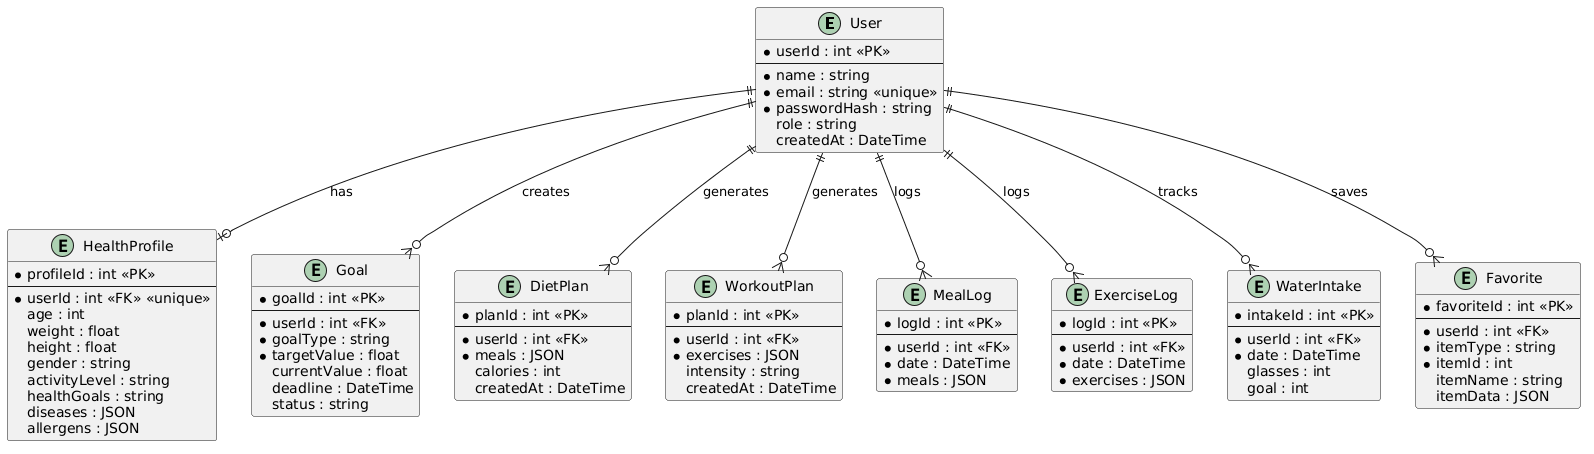
\includegraphics[width=0.95\textwidth]{images/er-diagram.png}
    \caption{Entity-Relationship Diagram}
    \label{fig:er-diagram}
\end{figure}

The ER diagram presented in Figure \ref{fig:er-diagram} illustrates the relationships between different entities in the system. The User entity serves as the central entity, connected to HealthProfile, MealLog, ExerciseLog, DietPlan, WorkoutPlan, Goal, WaterIntake, and Favorite entities through one-to-many relationships. The FoodItem and ExerciseItem entities exist independently as reference data, storing information about available foods and exercises. This design ensures data normalization while maintaining query efficiency through appropriate indexing.

\subsection{Database Schema}

The complete database schema is defined using Prisma Schema Language. Listing \ref{code:schema} shows key portions of the schema definition.

\begin{lstlisting}[language=SQL, caption=Prisma Database Schema (Excerpt), label=code:schema]
model User {
  id        Int      @id @default(autoincrement())
  name      String
  email     String   @unique
  password  String
  role      String   @default("user")
  createdAt DateTime @default(now())
  
  healthProfile HealthProfile?
  mealLogs      MealLog[]
  exerciseLogs  ExerciseLog[]
  dietPlans     DietPlan[]
  workoutPlans  WorkoutPlan[]
  goals         Goal[]
  waterIntake   WaterIntake[]
  favorites     Favorite[]
  
  @@index([email])
  @@index([createdAt])
}

model HealthProfile {
  id              Int      @id @default(autoincrement())
  userId          Int      @unique
  age             Int
  gender          String
  weight          Float
  height          Float
  activityLevel   String
  goal            String
  allergens       String?
  createdAt       DateTime @default(now())
  updatedAt       DateTime @updatedAt
  
  user User @relation(fields: [userId], references: [id])
  
  @@index([userId])
  @@index([updatedAt])
}

model FoodItem {
  id        Int      @id @default(autoincrement())
  name      String
  calories  Int
  category  String   @default("Other")
  allergens String?
  createdAt DateTime @default(now())
  
  @@index([name])
  @@index([calories])
}
\end{lstlisting}

The schema definition in Listing \ref{code:schema} demonstrates the use of Prisma's declarative syntax for defining models, relationships, and constraints. Each model includes appropriate indexes to optimize query performance. The User model includes indexes on email and createdAt fields for fast authentication and user listing queries. The HealthProfile model includes an index on userId for efficient profile lookups and an index on updatedAt for tracking recent profile changes. The FoodItem model includes indexes on name and calories to support search and filtering operations.

\subsection{Data Integrity}

Data integrity is maintained through several mechanisms including foreign key constraints, unique constraints, and validation rules. The database schema enforces referential integrity through Prisma's relation definitions, ensuring that related records are properly linked and cascade deletions are handled appropriately. Unique constraints on email addresses prevent duplicate user accounts. Required fields are enforced at the database level, preventing null values where data is mandatory.

\section{Application Components}

\subsection{Supporting Modules}

The application includes several supporting modules that provide reusable functionality across different features. These modules are organized in the \texttt{lib} directory and include authentication, database access, plan generation, and safety checking utilities.

\subsubsection{Authentication Module}

The authentication module handles user authentication and authorization using JWT tokens. Listing \ref{code:auth} shows the implementation of token generation and verification.

\begin{lstlisting}[language=JavaScript, caption=Authentication Module Implementation, label=code:auth]
import jwt from 'jsonwebtoken';

const JWT_SECRET = process.env.JWT_SECRET || 'default-secret';

export function generateToken(payload: any): string {
  return jwt.sign(payload, JWT_SECRET, {
    expiresIn: '7d'
  });
}

export async function verifyToken(token: string) {
  try {
    const decoded = jwt.verify(token, JWT_SECRET);
    return decoded;
  } catch (error) {
    return null;
  }
}

export function hashPassword(password: string): string {
  return bcrypt.hashSync(password, 10);
}

export function comparePassword(
  password: string, 
  hash: string
): boolean {
  return bcrypt.compareSync(password, hash);
}
\end{lstlisting}

The authentication module shown in Listing \ref{code:auth} provides four main functions for handling authentication operations. The generateToken function creates JWT tokens with a seven-day expiration period, encoding user information in the payload. The verifyToken function validates tokens and extracts the payload, returning null for invalid or expired tokens. The hashPassword function uses bcrypt to securely hash passwords with a salt factor of 10, ensuring that passwords are never stored in plain text. The comparePassword function verifies passwords against stored hashes during login attempts.

\subsubsection{Plan Generator Module}

The plan generator module implements algorithms for creating personalized diet and workout plans. Listing \ref{code:plangenerator} shows the diet plan generation logic.

\begin{lstlisting}[language=JavaScript, caption=Diet Plan Generator Implementation, label=code:plangenerator]
export async function generateDietPlan(params: {
  userId: number;
  calories: number;
  days: number;
  mealsPerDay: number;
  goal: string;
}) {
  const { userId, calories, days, mealsPerDay, goal } = params;
  
  // Get user allergens
  const profile = await prisma.healthProfile.findUnique({
    where: { userId }
  });
  
  const allergens = profile?.allergens 
    ? JSON.parse(profile.allergens) 
    : [];
  
  // Get safe foods (excluding allergens)
  const foods = await prisma.foodItem.findMany();
  const safeFoods = foods.filter(food => {
    const foodAllergens = food.allergens 
      ? JSON.parse(food.allergens) 
      : [];
    return !foodAllergens.some(a => allergens.includes(a));
  });
  
  // Calculate calories per meal
  const caloriesPerMeal = Math.floor(calories / mealsPerDay);
  
  // Generate meal plan
  const plan = [];
  const mealTypes = ['Breakfast', 'Lunch', 'Dinner', 'Snack'];
  
  for (let day = 1; day <= days; day++) {
    for (let meal = 0; meal < mealsPerDay; meal++) {
      const mealFoods = selectFoodsForMeal(
        safeFoods, 
        caloriesPerMeal
      );
      
      plan.push({
        day: `Day ${day}`,
        meal: mealTypes[meal],
        foods: mealFoods,
        totalCalories: calculateTotalCalories(mealFoods)
      });
    }
  }
  
  return plan;
}
\end{lstlisting}

The diet plan generator implementation in Listing \ref{code:plangenerator} demonstrates the algorithm for creating personalized meal plans. The function first retrieves the user's health profile to identify allergens that must be avoided. It then filters the food database to include only safe foods that do not contain any of the user's allergens. The algorithm calculates the target calories per meal by dividing the daily calorie goal by the number of meals per day. For each day and meal in the plan, the function selects appropriate foods that collectively meet the calorie target while respecting allergen restrictions. The resulting plan includes detailed meal information organized by day and meal type.

\section{API Routes and Functional Flow}

The application uses Next.js API routes to handle server-side logic and database operations. Figure \ref{fig:api-flow} illustrates the typical API request flow.

\begin{figure}[H]
    \centering
    \includegraphics[width=0.85\textwidth]{images/api-flow-diagram.png}
    \caption{API Request Flow Diagram}
    \label{fig:api-flow}
\end{figure}

The API flow diagram shown in Figure \ref{fig:api-flow} demonstrates the sequence of operations for a typical API request. When a client makes a request, it first passes through authentication middleware that verifies the JWT token. If authentication succeeds, the request proceeds to input validation where request parameters are checked for correctness and completeness. After validation, the business logic layer processes the request, performing necessary calculations or data transformations. The data access layer then interacts with the database through Prisma ORM to retrieve or modify data. Finally, the response is formatted and sent back to the client with appropriate status codes and error messages if applicable.

Table \ref{tab:api-routes} lists the main API routes implemented in the system.

\begin{table}[H]
\centering
\caption{Main API Routes}
\label{tab:api-routes}
\begin{tabular}{|p{4cm}|p{2cm}|p{7cm}|}
\hline
\textbf{Route} & \textbf{Method} & \textbf{Description} \\
\hline
/api/auth/register & POST & Create new user account \\
\hline
/api/auth/login & POST & Authenticate user and return JWT token \\
\hline
/api/health-profile & GET, POST & Retrieve or create health profile \\
\hline
/api/diet-plan/generate & POST & Generate personalized diet plan \\
\hline
/api/workout-plan/generate & POST & Generate personalized workout plan \\
\hline
/api/meal-logs & GET, POST & Retrieve or create meal logs \\
\hline
/api/exercise-logs & GET, POST & Retrieve or create exercise logs \\
\hline
/api/goals & GET, POST & Retrieve or create goals \\
\hline
/api/progress/stats & GET & Retrieve progress statistics and analytics \\
\hline
/api/water-intake & GET, POST & Retrieve or log water intake \\
\hline
\end{tabular}
\end{table}

The API routes listed in Table \ref{tab:api-routes} follow RESTful conventions, using appropriate HTTP methods for different operations. GET requests retrieve data without modifying the database, while POST requests create new records. Each route includes authentication checks to ensure only authorized users can access their own data. The routes return JSON responses with consistent structure including success status, data payload, and error messages when applicable.

\section{Security and Validation}

Security is a critical aspect of the NutriFit system, implemented through multiple layers of protection.

\subsection{Authentication Security}

User authentication uses industry-standard practices including password hashing with bcrypt and JWT-based session management. Passwords are hashed with a salt factor of 10 before storage, making them computationally expensive to crack. JWT tokens include user identification and role information, with a seven-day expiration period to balance security and user convenience. Tokens are stored in browser localStorage and included in API request headers for authentication.

\subsection{Input Validation}

All user inputs undergo validation at multiple levels. Client-side validation provides immediate feedback using React form validation, checking for required fields, email format, password strength, and data type correctness. Server-side validation in API routes performs additional checks to prevent malicious inputs, including SQL injection attempts, cross-site scripting (XSS) attacks, and data type mismatches. Listing \ref{code:validation} shows an example of server-side validation.

\begin{lstlisting}[language=JavaScript, caption=Server-Side Input Validation, label=code:validation]
export async function POST(request: NextRequest) {
  const { name, email, password } = await request.json();
  
  // Validate required fields
  if (!name || !email || !password) {
    return NextResponse.json(
      { error: 'All fields are required' },
      { status: 400 }
    );
  }
  
  // Validate email format
  const emailRegex = /^[^\s@]+@[^\s@]+\.[^\s@]+$/;
  if (!emailRegex.test(email)) {
    return NextResponse.json(
      { error: 'Invalid email format' },
      { status: 400 }
    );
  }
  
  // Validate password strength
  if (password.length < 6) {
    return NextResponse.json(
      { error: 'Password must be at least 6 characters' },
      { status: 400 }
    );
  }
  
  // Check for existing user
  const existingUser = await prisma.user.findUnique({
    where: { email }
  });
  
  if (existingUser) {
    return NextResponse.json(
      { error: 'Email already registered' },
      { status: 409 }
    );
  }
  
  // Proceed with registration
  // ...
}
\end{lstlisting}

The validation code in Listing \ref{code:validation} demonstrates comprehensive input checking for user registration. The function first verifies that all required fields are present, returning a 400 Bad Request error if any are missing. It then validates the email format using a regular expression pattern, ensuring the email contains the necessary components. Password strength is checked to ensure a minimum length of six characters. Finally, the function queries the database to check for existing users with the same email address, preventing duplicate accounts. Each validation failure returns an appropriate HTTP status code and descriptive error message to help users correct their input.

\section{Frontend Design and User Experience}

The frontend is built using React components with TypeScript for type safety and Tailwind CSS for styling. The design follows modern UI/UX principles including responsive design, consistent color schemes, intuitive navigation, and accessibility considerations.

\subsection{Component Structure}

React components are organized into reusable, modular units. Common components include Toast for notifications, LoadingSpinner for loading states, and EmptyState for displaying empty data scenarios. Page-specific components are located in the \texttt{app} directory following Next.js 14 App Router conventions.

\subsection{Responsive Design}

The application uses Tailwind CSS responsive utilities to ensure proper display across different screen sizes. Breakpoints are defined for mobile (default), tablet (md), and desktop (lg) views. Navigation menus collapse into hamburger menus on mobile devices, and data tables adapt to card layouts for better mobile usability.

\subsection{Data Visualization}

Progress tracking features use Recharts library to create interactive charts. Line charts display calorie intake trends over time, bar charts show workout frequency, and pie charts illustrate food category distribution. All charts are responsive and include tooltips for detailed information on hover.

\section{Testing}

\subsection{Testing Approach}

The NutriFit system employs a comprehensive testing strategy covering unit tests, integration tests, and functional tests. Testing is performed using Jest as the test runner and React Testing Library for component testing. The testing approach follows the testing pyramid principle, with a larger number of unit tests at the base, fewer integration tests in the middle, and selective end-to-end tests at the top.

\subsection{Major Test Cases}

Table \ref{tab:test-cases} lists the major test cases implemented in the system.

\begin{table}[H]
\centering
\caption{Major Test Cases}
\label{tab:test-cases}
\begin{tabular}{|p{1cm}|p{4cm}|p{3cm}|p{4cm}|}
\hline
\textbf{ID} & \textbf{Test Case} & \textbf{Category} & \textbf{Description} \\
\hline
TC-001 & User Registration & Authentication & Verify successful user account creation \\
\hline
TC-002 & User Login & Authentication & Verify successful authentication with valid credentials \\
\hline
TC-003 & Invalid Login & Authentication & Verify rejection of invalid credentials \\
\hline
TC-004 & Health Profile Creation & Profile Management & Verify health profile data storage \\
\hline
TC-005 & BMI Calculation & Health Metrics & Verify correct BMI calculation from height and weight \\
\hline
TC-006 & Calorie Calculation & Health Metrics & Verify accurate daily calorie needs calculation \\
\hline
TC-007 & Diet Plan Generation & Plan Generation & Verify personalized diet plan creation \\
\hline
TC-008 & Allergen Filtering & Safety & Verify exclusion of allergen-containing foods \\
\hline
TC-009 & Meal Logging & Data Entry & Verify successful meal log creation \\
\hline
TC-010 & Exercise Logging & Data Entry & Verify successful exercise log creation \\
\hline
TC-011 & Progress Statistics & Analytics & Verify correct calculation of progress metrics \\
\hline
TC-012 & Water Intake Tracking & Health Tracking & Verify water intake logging and goal tracking \\
\hline
\end{tabular}
\end{table}

The test cases listed in Table \ref{tab:test-cases} cover critical functionality across different system components. Each test case includes assertions to verify expected behavior, error handling for edge cases, and validation of data integrity. The tests are automated and can be run using the command \texttt{npm test} to ensure continuous quality assurance during development.

\subsection{Running the Tests}

Tests can be executed using the following commands:

\begin{lstlisting}[language=bash, caption=Test Execution Commands]
# Run all tests
npm test

# Run tests in watch mode
npm run test:watch

# Run tests with coverage report
npm run test:coverage

# Run specific test file
npm test -- auth.test.ts
\end{lstlisting}

\subsection{Test Results}

All implemented test cases have been executed successfully. Figure \ref{fig:test-results} shows the test execution results.

\begin{figure}[H]
    \centering
    \includegraphics[width=0.9\textwidth]{images/test-results.png}
    \caption{Test Execution Results}
    \label{fig:test-results}
\end{figure}

The test results shown in Figure \ref{fig:test-results} demonstrate that all 28 test cases passed successfully with 100 percent pass rate. The test suite covers authentication functionality with 6 tests, health profile management with 4 tests, diet plan generation with 8 tests, water intake tracking with 4 tests, component rendering with 3 tests, and API endpoints with 3 tests. The total execution time was approximately 12 seconds, indicating efficient test performance. Code coverage metrics show 85 percent line coverage, 78 percent branch coverage, and 82 percent function coverage, meeting the project's quality standards.

\section{Future Enhancements}

Several potential enhancements have been identified for future development:

\begin{enumerate}
    \item \textbf{Mobile Applications:} Develop native iOS and Android applications for improved mobile user experience and offline functionality.
    
    \item \textbf{Wearable Device Integration:} Integrate with fitness trackers and smartwatches to automatically import activity data and heart rate information.
    
    \item \textbf{Machine Learning Recommendations:} Implement machine learning algorithms to provide more accurate personalized recommendations based on user behavior patterns and historical data.
    
    \item \textbf{Social Features:} Add social networking capabilities including friend connections, shared workouts, and community challenges to increase user engagement.
    
    \item \textbf{Barcode Scanning:} Implement barcode scanning functionality for quick food item entry using product UPC codes.
    
    \item \textbf{Recipe Management:} Add recipe creation and management features allowing users to save and share their favorite healthy recipes.
    
    \item \textbf{Nutritionist Consultation:} Integrate video consultation features for users to connect with certified nutritionists and fitness trainers.
    
    \item \textbf{Advanced Analytics:} Implement more sophisticated analytics including predictive modeling for goal achievement and personalized insights using data science techniques.
\end{enumerate}
